\documentclass[a4paper,12pt]{article}
\usepackage{ucs}
\usepackage[utf8x]{inputenc}
\usepackage{amsfonts}
\usepackage[english,russian]{babel}
\usepackage[T1, T2A]{fontenc}
\frenchspacing
\usepackage{amsmath,amssymb,amsthm}
\usepackage[a4paper, margin=1in]{geometry}
\usepackage{fontspec}
\usepackage{noto}
\usepackage[table]{xcolor}
\usepackage{multirow}
\usepackage{diagbox}
\usepackage{graphicx}
\usepackage{listings}
\usepackage{minted}
\usepackage[obeyspaces]{xurl}
\usepackage{hyperref}
\usepackage{bm}
\usepackage{pdfpages}
\graphicspath{ {./img/} }
\renewcommand{\baselinestretch}{1.1}
\renewcommand{\arraystretch}{1.1}


\newtheorem{name}{Printed output}
\newtheorem{problem}{Задача}
\newenvironment{solution}{\renewcommand{\proofname}{\unskip\indent\nopunct}\begin{proof}}{\end{proof}}

\numberwithin{equation}{section}


\begin{document}

\sloppy

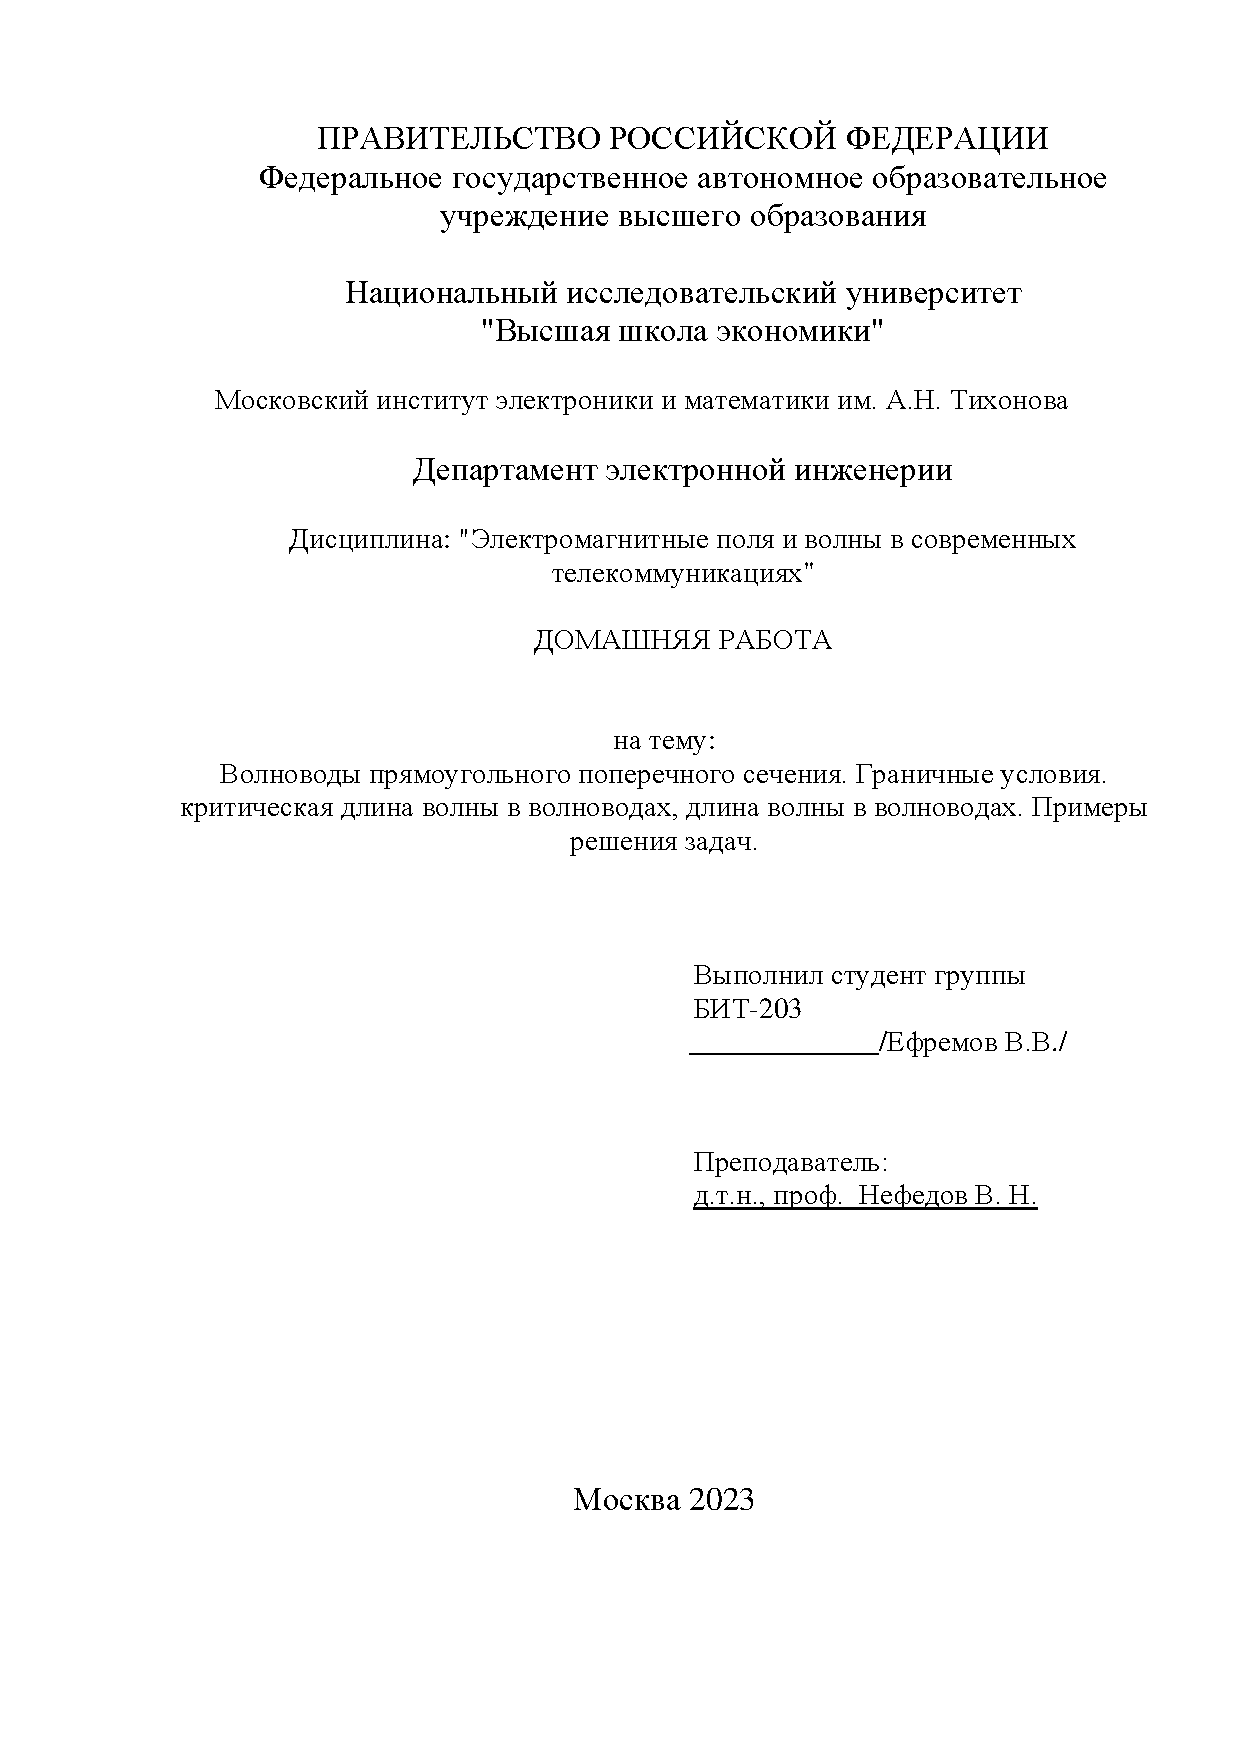
\includepdf[pages=-]{title.pdf}


\tableofcontents


\section{Предисловие}
Эта работа относительно короткая из-за того, что я плохо планировал и писал в последний момент.
Также я затрудняюсь найти хороших задач на тему работы, поэтому взял только одну (да и ту не сильно содержательную).

\section{Теория}
Рассматривая волновод, часто предполагают что это бесконечный цилиндр, т.е. имеет одинаковую форму сечения на всем протяжении.
Также удобно выбрать систему координат так, чтобы ось $Oz$ была направлена вдоль волновода.
Для прямоугольных волноводов ось $Ox$ направляют вдоль большей стороны, $Oy$ - вдоль меньшей.
Будем придерживаться тех же соглашений.

\begin{center}
    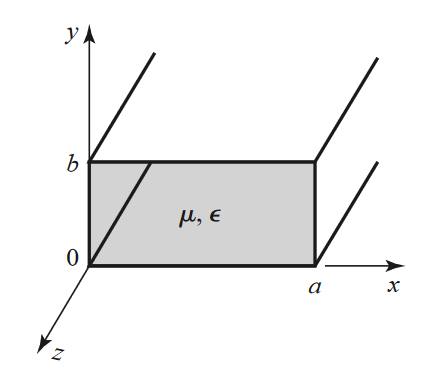
\includegraphics[width=8cm]{1.png}
\end{center}

Также часто отдельно выделяют три вида полей, т.к. они заметно проще для рассмотрения.

TEM (transverse electromagnetic wave) - $E_z = 0, H_z = 0$, т.е. оба вектора и электрического, и магнитного полей лежат целиком в плоскости перпендикулярной оси волновода.

TE - только $E_z = 0$.

TM - только $H_z = 0$.

\subsection{Граничные условия}
Граничные условия, вообще говоря, не зависят от формы волновода.
Требуется лишь чтобы тангенциальная/касательная составляющая электрического поля $E$ и нормальная составляющая магнитного поля $B$ были равны нулю на границе волновода.

\subsection{Критическая длина волны}
Волноводы имеют, так называемую, критическую частоту (cut-off frequency).
Волна частоты ниже критической не распространяется в воноводе.
Более точно - она экспоненциально затухает.

Если говорить о том почему так получается, то нужно обратиться к уравнениям.
Если положить, что поля менются по синусоидальному закону, то из уравнений Максвелла получется уравнение Гемгольтца
$$\nabla \vec{L} + k^2 \vec{L} = 0$$
Где, $\vec{L}$ либо электрическая, либо магнитная составляющие поля.

Это уравнение решается известным методом разделения переменных (положим что $L(x, y, z) = X(x) Y(y) Z(z)$, т.е. что неизвестная функция разлагается в произведение компонент, каждая из которых зависит только от одной координаты; после такой замеы уравнение распадется на три отдельных уравнения на функции одной переменной, которые легко решаются).

Сами решения не так важны, важно соотношение на один из параметров решения
$$\beta = \sqrt{k^2 - \left(\frac{m\pi}{a}\right)^2 - \left(\frac{n\pi}{b}\right)^2}$$
$\beta$ - фазовая постоянная, часть постоянной распространения - $\gamma = \alpha + j\beta$.

При малых $k$, выражение под корнем становится отрицательным, $\beta$ мнимым, и в $\gamma$ появляется действительная часть, постоянная ослабления, которая и указывает на то, что волная экспоненциально затухает.

Аккуратное выражение для критической частоты
\begin{equation} \label{eq:fcmn}
    f_{c_{mn}}= \frac{c}{2\pi \sqrt{\mu \varepsilon}} \sqrt{\left(\frac{m\pi}{a}\right)^2 + \left(\frac{n\pi}{b}\right)^2}
\end{equation}

Здесь $m, n$ - это некоторые целые, неотрицательные числа.
Их можно считать параметрами, т.к. в волноводе может распространяться целое семейство волн.


\section{Примеры задач}

\begin{problem}
{\normalfont \cite[p.~116, Example 3.1]{Pozar:882338}}
Рассмотрим отрезок медного волновода заполненного тефлоном с размерами $1.07$ см на $0.43$ см.
Найдите критическую частоту для волны $TE_{11}$.
\end{problem}
\begin{solution}
Диэлектрическая проницаемость тефлона $\varepsilon = 2.08$, магнитную проницаемость меди будем считать равной единице.
Подставляя числа в уравнение \ref{eq:fcmn}, получаем
\begin{equation}
    f_{c_11} = \frac{299 792 458}{2 \pi \sqrt{1 \cdot 2.08}} \sqrt{\left(\frac{\pi}{0.0107}\right)^2 + \left(\frac{\pi}{0.0043}\right)^2} \approx 26.05~\text{ГГц}
\end{equation}

\end{solution}



\section{Литература}
\renewcommand\refname{\vskip -1cm}
\bibliographystyle{plain}
\bibliography{refs}


\end{document}
